\documentclass[a4paper]{scrartcl}
%pre\'ambulo

\usepackage{fullpage}
\usepackage{lmodern}
\usepackage[spanish,activeacute]{babel}
\usepackage[T1]{fontenc}

\usepackage{xcolor}
\usepackage{listings}
\lstset{ 
	basicstyle=\ttfamily,
	showstringspaces=false,
	commentstyle=\color{red},
	keywordstyle=\color{blue}
}

\usepackage{graphicx}

\title{SSH\_Intro\_v01}
\author{Facundo Navarro}

\begin{document}
%cuerpo del documento

\maketitle
\section{SSH - Introducci'on}
SSH o Secure Shell, es un protocolo de administraci'on para acceder de forma remota a un servidor privado, el acceso se grarantiza mediante el uso de una clave p'ublica y una clave privada mediante un cifrado criptogr'afico asim'etrico tambien llamado criptograf'ia de clave p'ublica o criptograf'ia de dos claves. El m'etodo consiste en crear un par de llaves, que mediante los m'etodos cript'ograficos se garantiza que esa pareja de claves s'olo se puede generar una vez, de modo que se puede asumir que no es posible que dos personas hayan obtenido casualmente la misma pareja de claves.

La clave p'ublica se puede entregar a cualquier persona y es la que permanece en el servidor, la otra clave es la clave privada y el propietario debe guardarla de modo que nadie tenga acceso a ella.

\subsection{Generaci'on de par de claves SSH en sistemas UNIX}
Un par de llaves SSH puede ser generado ejecuando el comando \textit{ssh-keygen} dentro de la terminal, el cual por defecto usa seguridad 2048-bit RSA, luego de presionado se pedir'a que se indique un nombre de archivo como asi tambi'en la ruta, si se deja vac'io el mismo se guardar'a en la ruta \textit{/home/usuario/.ssh/} con el nombre \textit{id\_rsa} (clave privada) e \textit{id\_rsa.pub} (clave p'ublica), como se puede observar en las im'agenes {\color{blue}\ref{fig:1}} y {\color{blue}\ref{fig:2}}.

\begin{figure}[ht]
  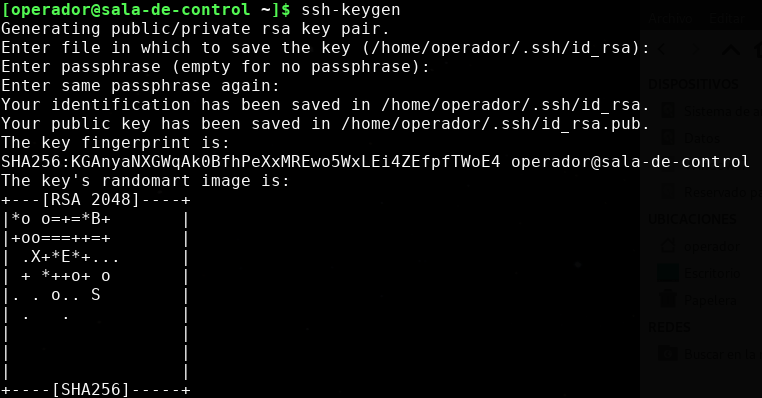
\includegraphics[width=\columnwidth]{./ssh_intro_imgs/A}
  \caption{Salida terminal dejando vac'io tanto el nombre del archivo como el \textit{passphrase}}
  \label{fig:1}
\end{figure}

\begin{figure}[ht]
  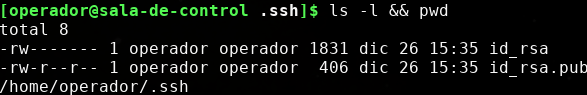
\includegraphics[scale=0.5]{./ssh_intro_imgs/B}
  \caption{Directorio en \$HOME/.ssh/ se ve las claves \textit{id\_rsa} e \textit{id\_rsa.pub}}
  \label{fig:2}
\end{figure}

De igual manera se recomienda utilizar la encirptaci'on de 4096 bits, como asi tambi'en no dejar en blanco la \textit{passphrase} para la clave privada de forma que por cualquier motivo se obtenga la clave privada esta quede encriptada con la \textit{passphrase} y no pueda ser utilizada, cabe aclarar que esta contrase'na no la debe proporcionar por ningun motivo, en caso de olvido se deber'a generar un nuevo par de claves, el comando recomendado a ejecutar es el siguiente:
\begin{lstlisting}[language=bash]
$ ssh-keygen -f <filename> -t rsa -b 4096 -C "email@dominio.com"
\end{lstlisting}

\begin{description}
	\item[-f] especifica el nombre del archivo como as'i tambi'en la ruta en donde se guardar'a.
	\item[-t] indica el algoritmo a utilizar.
	\item[-b] indica el tama'no o cantidad de bits.
	\item[-C] es importante a'nadir un comentario acorde de manera de identificar el propietario de la clave p'ublica por parte del administrador en caso de extrav'io.
\end{description}
En la imagen {\color{blue}\ref{fig:3}} se puede observar el procedimiento completo, en primer lugar creamos un directorio llamado \textit{llave\_cluster}, luego se ejecuta el comando dado previamente reemplazando adecuadamente con nuestros datos, el nombre que eleg'i para el par de llaves es \textit{fnavarro}
\begin{figure}[!ht]
  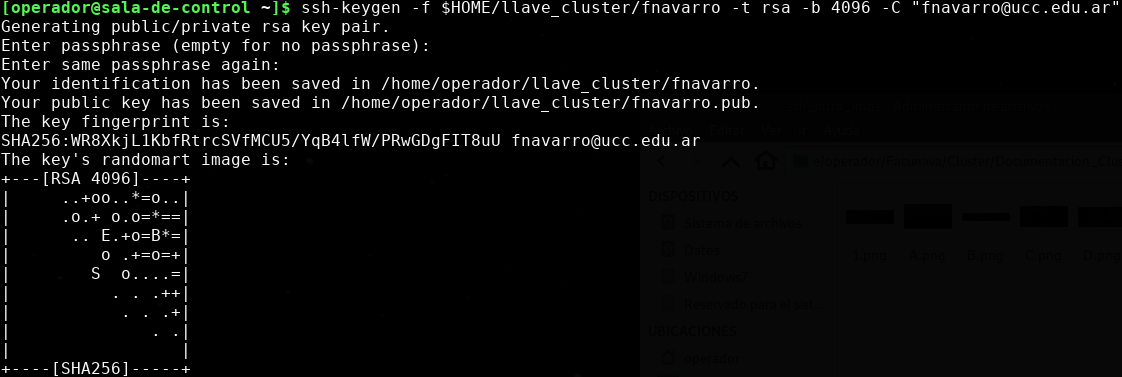
\includegraphics[scale=0.38]{./ssh_intro_imgs/C}
  \caption{}
  \label{fig:3}
\end{figure}

En la imagen {\color{blue}\ref{fig:4}} se ve que se crearon dentro del directorio especificado, un archivo \textit{fnavarro} (clave privada) y otro de mismo nombre pero de extensi'on \textit{.pub} (clave p'ublica).
\begin{figure}[!ht]
  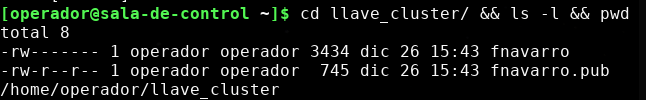
\includegraphics[scale=0.5]{./ssh_intro_imgs/D}
  \caption{Par de llaves creadas acorde al parametro \textbf{-f}}
  \label{fig:4}
\end{figure}

\subsection{Accediendo al Cluster Navira}
Una vez que se han generado y enviado la clave p'ublica al administrador \textit{(it.ing@ucc.edu.ar)} y este le haya confirmado la creaci'on de su usuario, se podra acceder al cluster por SSH desde la terminal de la siguiente manera:

\begin{lstlisting}[language=bash]
$ ssh <usuario>@navira.cidie.ucc.edu.ar -p 2230
\end{lstlisting}

es impresindible la bandera \textbf{-p 2230} ya que es el puerto asignado por parte de servicio t'ecnico para el acceso desde el exterior.

\begin{figure}[ht]
  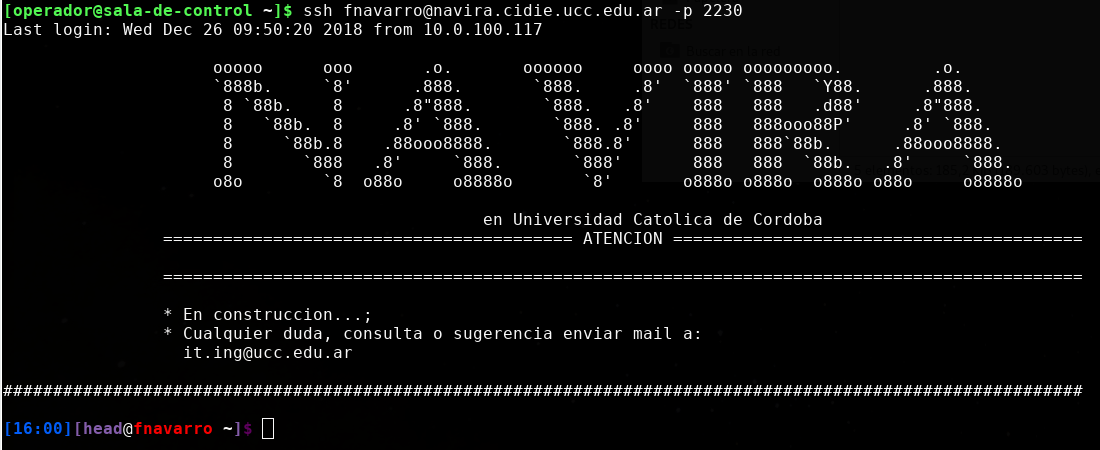
\includegraphics[width=\columnwidth]{./ssh_intro_imgs/E}
  \caption{}
  \label{fig:5}
\end{figure}

\end{document}
